\documentclass[10pt,a4paper,twocolumn]{article}
\usepackage{graphicx} 
\usepackage[labelformat=empty]{caption}
\usepackage{import}
\usepackage[T2A]{fontenc}
\usepackage[margin=1.5cm,top=1.5cm]{geometry}
\usepackage[english,russian]{babel}
\title {\textbf{Pасчетная работа}}
\author{Мацукевич Захар 421703}
\date{}
\begin{document}
\maketitle
\large{\hspace{-0.4cm}\textbf{Цель:}}
\par Продемонстрировать работу программы решения теоретико-графовой задачи по построению дерева кротчайших путей заданного графа.
\\ \large{\textbf {Ключевые понятия:}}
\par Граф – совокупность двух множеств — множества самих объектов (вершин) и множества их парных связей (ребер).
\par Ориентированный граф (кратко орграф) — граф, рёбрам которого присвоено направление.
\par Путь в графе – это последовательность рёбер, в которой конец каждого ребра (кроме последнего) совпадает с началом следующего. 
\par Список смежности - один из способов представления графа в виде коллекции списков вершин. Каждой вершине графа соответствует список, состоящий из «соседей» этой вершины.
\par Матрица смежности - это вид представления графа в виде матрицы, когда пересечение столбцов и строк задаёт дуги.
\par Неориентированный граф — граф, в котором рёбра не имеют направления. На рисунке выше показан как раз неориентированный граф. В таком неориентированном графе можно перемещаться вдоль ребра в любом из двух направлений.
\par Взвешанный граф - граф, ребра которого имеют некое числовое значение.
\par Дерево кратчайших путей — подграф исходного графа, одна из вершин которого является вершиной, кратчайшие пути из которой хранит граф, в котором каждый путь от корня до любой другой вершины является кратчайшим в исходном графе.
\par \large{\hspace{-0.6cm}\textbf{Демонстрация работы программы в семантической памяти на примере невзвешенного неориентированного графа:}}
\par Для лучшего восприятия картинок ненужные на соответвтующем этапе эл-ты SCg будут скрыты. Каждому пункту соответствует рисунок с соответствующим номером.
\begin{enumerate}
% 1
	\item Задаем сам граф, его принадлежность к множеству графов и непринадлежность к множествам ориентированных и взвешенных графов, а также для всех его вершин и ребер указываем принадлежность к соответствующим множествам. Указываем начальную вершину, пусть это будет вершина ``1''. Отметим её же посещенной, указав принадлежность к соответствующему множеству.
	\begin{figure}[h!]
		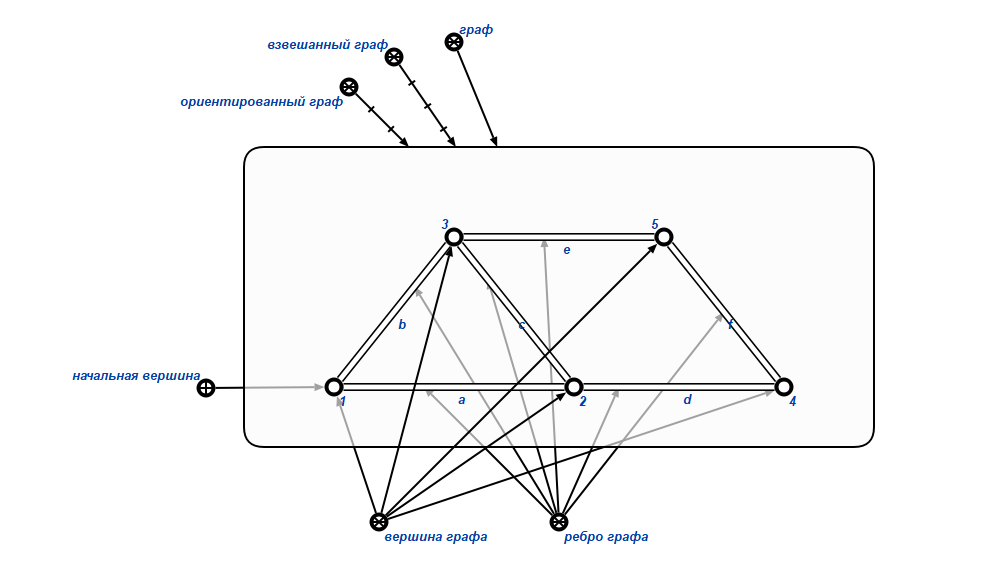
\includegraphics[width=0.5\textwidth]{img/img1.png}
		\caption{Рис.1}
	\end{figure}
% 2
	\item Начать следует с первой вершины. Зададим итерацию ``it1'' и присвоим ей все происходящее. Отметим вершину ``1'' как текущую вершину. Путь в не имеет ребер, т.к. изначально мы находимся в конце пути. Значит задаем элемент ``путь 1-1'' и указываем, что это объединение из вершины ``1'' и это граф. Также связываем вершину ``1'' с ``путь 1-1'' ролевым отношением ``путь сюда*''.
	\begin{figure}[h!]
		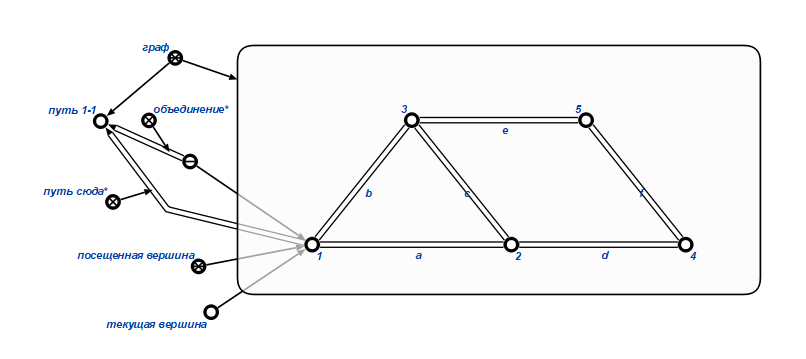
\includegraphics[width=0.5\textwidth]{img/img2.png}
		\caption{Рис.2}
	\end{figure}
% 3
	\item Теперь нужно объединить выходящие из текущей вершины ребра и узлы, в которые они приходят, в структуру ``it<номер итерации>'' какое ребро к какому узлу ведет и связать структуры отношением ``следующая''. Указываем принадлежность вершины ``1'' к множеству пройденных вершин. Таким образом получаем очередность выполнения операций, зная ребро, по которому попали в каждый узел.  
	\begin{figure}[h]
		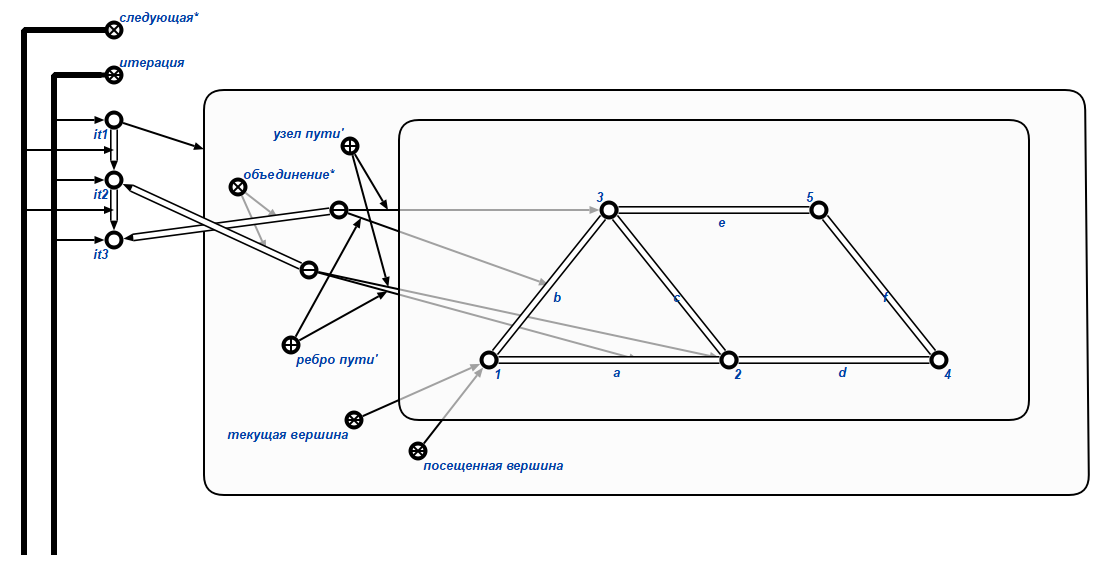
\includegraphics[width=0.45\textwidth]{img/img3.png}
		\caption{Рис.3}
	\end{figure}
% 4
	\item Закончив первую итерацию идем к следующей. Помечаем вершину пути как текущую. Если она помечена как пройденная, то ничего не делаем и идем к следующей итерации. Иначе объединяем текущую вершину, ребро пути и ``путь сюда*'' для вершины, с которой еще связано ребро пути, в данном случае - это вершина ``2'', ребро ``а'' и ``путь 1-1''. Результат объединения - ``путь 1-2''. Связываем ``путь 1-2'' с вершиной ``2'' отношением ``путь сюда*''. ``Путь 1-2'' также граф.
	\begin{figure}[h]
		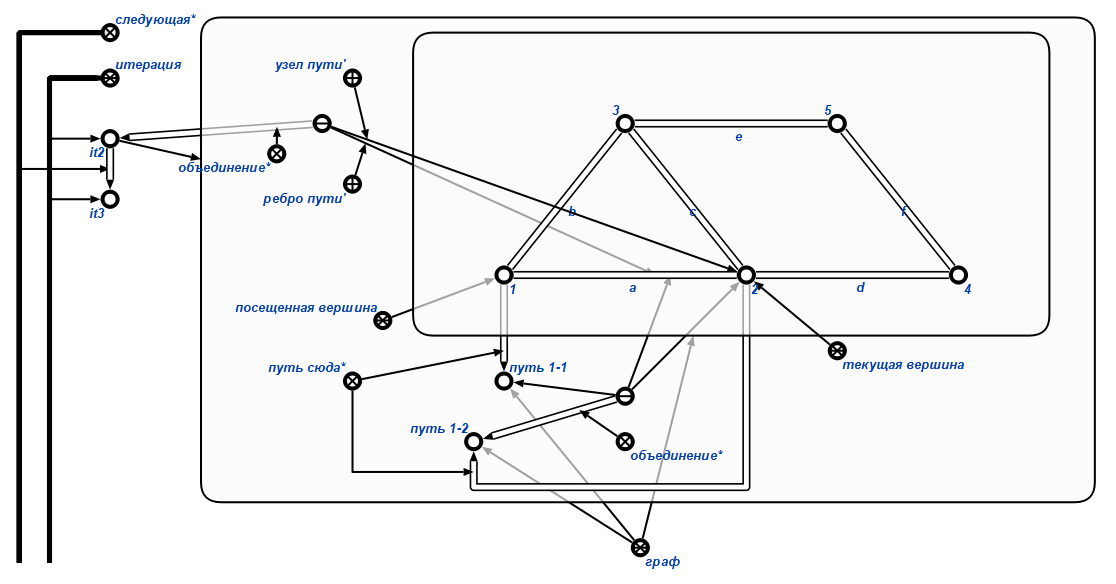
\includegraphics[width=0.45\textwidth]{img/img4.png}
		\caption{Рис.4}
	\end{figure}
% 5
	\item Теперь определим следующие итерации. Объединяем ребра ``c'' и ``d'' с вершинами ``3'' и ``4'' соответственно в итерации ``it4'' и ``it5'', обозначая ребра и вершины пути для каждой итерации. Помечаем ``2'' пройденной вершиной.
	\begin{figure}[h]
		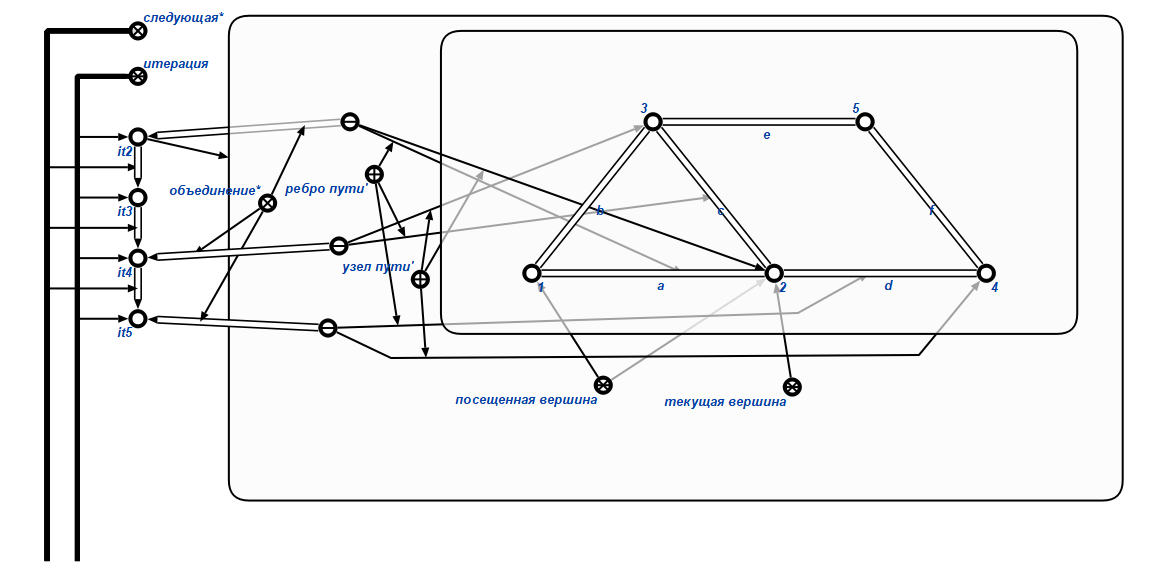
\includegraphics[width=0.45\textwidth]{img/img5.png}
		\caption{Рис.5}
	\end{figure}
    \newpage
% 6
	\item На третей итерации делаем все те же действия, что на итерации ``it2'': строим ``путь 1-3'' объединяя текущую вершину ``3'', ребро пути "b" и ``путь 1-1''.
	\begin{figure}[h]
		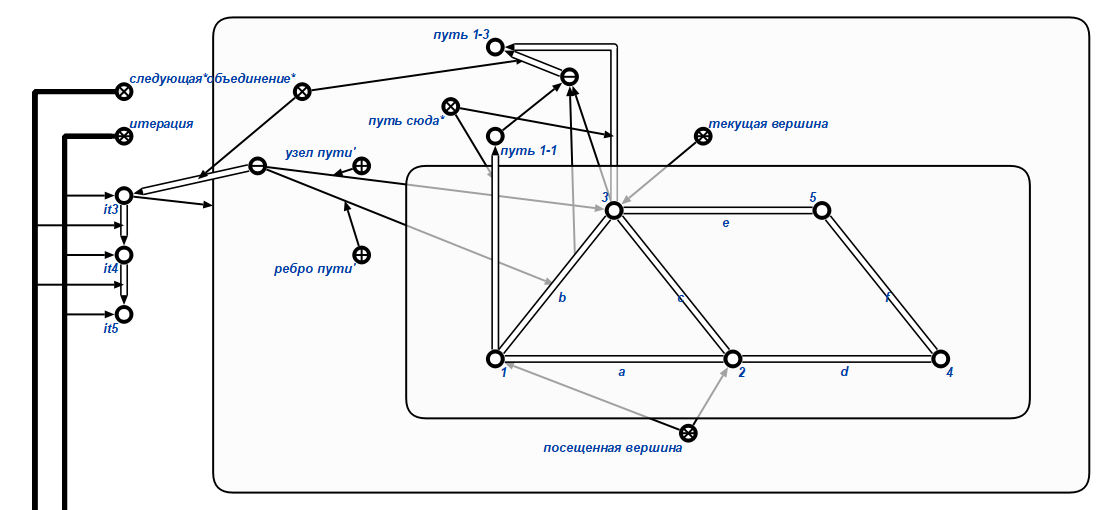
\includegraphics[width=0.45\textwidth]{img/img6.png}
		\caption{Рис.6}
	\end{figure}
% 7
	\item Определяем следующие итерации. Указываем узел ``3'' как посещенную вершину.
	\begin{figure}[h]
		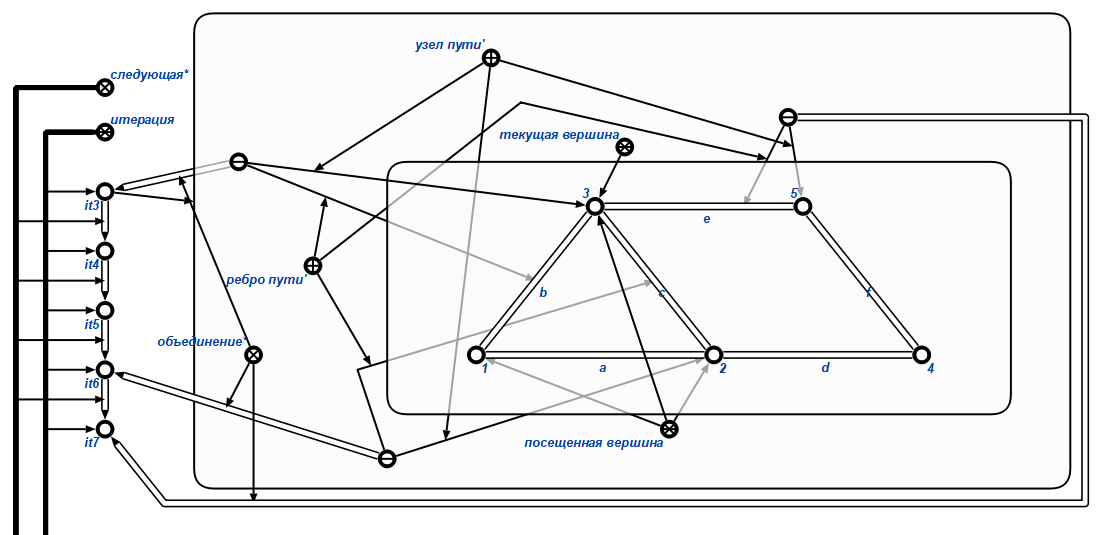
\includegraphics[width=0.45\textwidth]{img/img7.png}
		\caption{Рис.7}
	\end{figure}
% 8
	\item Итерация ``it4''- ребро ``с'' и вершина ``3''. Отмечаем её как текущую. Видим, что она уже принадлежит множеству посещенных вершин, так что никаких операций производить не нужно, кратчайший путь в эту вершину уже записан как ``путь 1-3''. Переходим к ``it5''.
    \newpage
    \begin{figure}[h]
		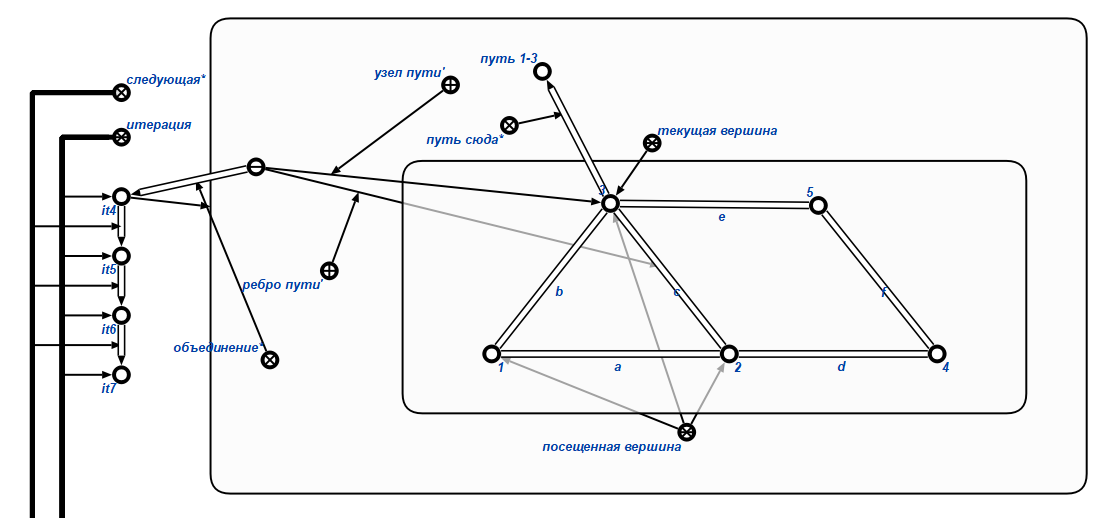
\includegraphics[width=0.45\textwidth]{img/img8.png}
		\caption{Рис.8}
	\end{figure}
% 9
	\item На пятой итерации рассматривается вершина ``4'' и ребро ``d''. Вершина ``4'' не была посещена, так что помечаем ее как текущую, объединяем вершину и ребро пути пятой итерации с путем ``путь 1-2'' в ``путь 1-4'' и указываем, что это ``путь сюда*'' для узла ``4''. 
	\begin{figure}[h]
		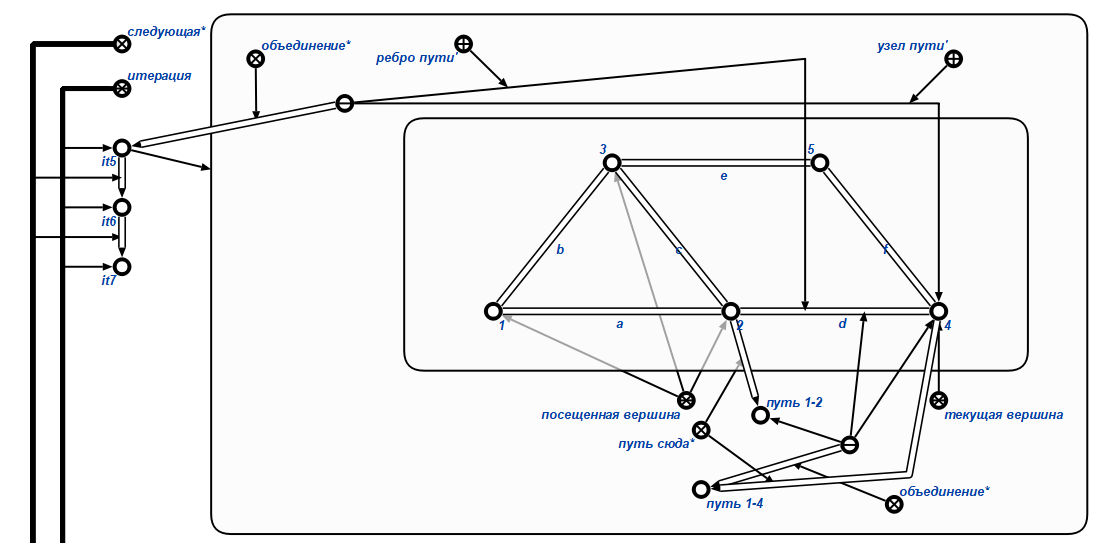
\includegraphics[width=0.45\textwidth]{img/img9.png}
		\caption{Рис.9}
	\end{figure}
% 10
	\item Объединяем ребро ``f'' и вершину ``5'' в следующую итерацию ``it8''. Помечаем ``4'' как посещенную вершину и идем дальше в очереди.
	\begin{figure}[h]
		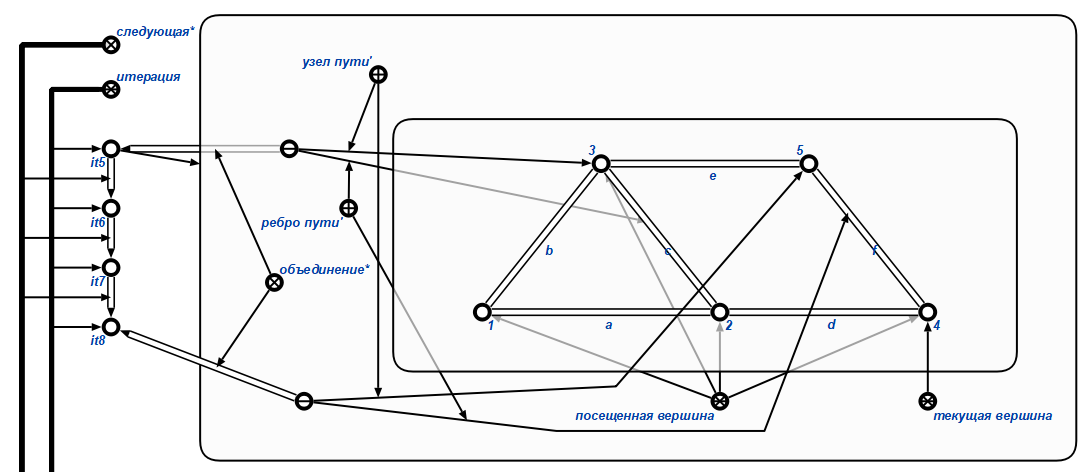
\includegraphics[width=0.45\textwidth]{img/img10.png}
		\caption{Рис.10}
	\end{figure}
% 11
	\item Итерация ``it6'' имеет вершину пути ``2'' и ребро пути ``c'', отмечаем вершину как текущую. Замечаем ее принадлежность множеству посещенных вершин и наличие связи ``путь сюда*'', значит игнорируем эту итерацию и идем дальше.
    \newpage
	\begin{figure}[h]
		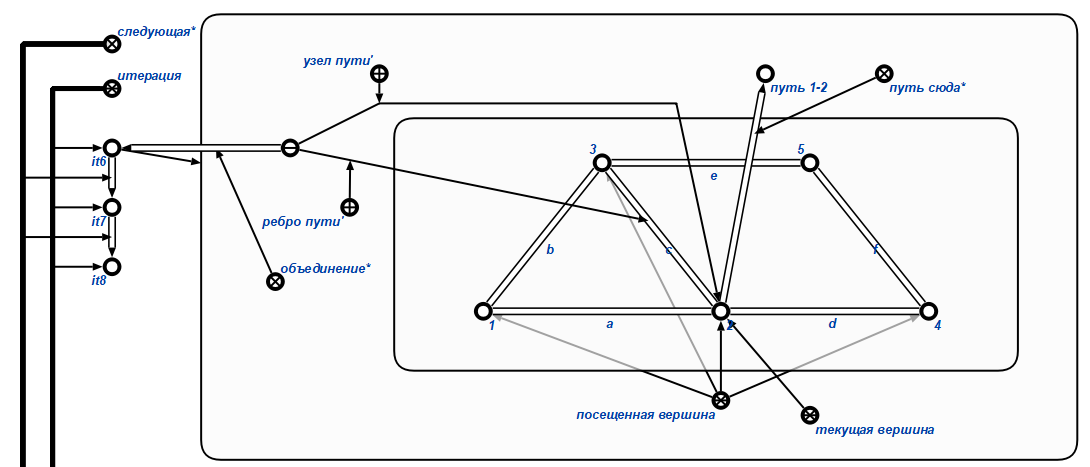
\includegraphics[width=0.45\textwidth]{img/img11.png}
		\caption{Рис.11}
	\end{figure}
% 12
	\item На седьмой итерации помечаем ``5'' как текущую вершину. Объединяем ребро пути ``e'', текущую вершину и ``путь 1-3'' в ``путь 1-5''. Объединяем ребро ``f'' и вершину ``4'' в ``it9''. Помечаем вершину ``5'' как посещенную и движемся дальше. 
	\begin{figure}[h]
		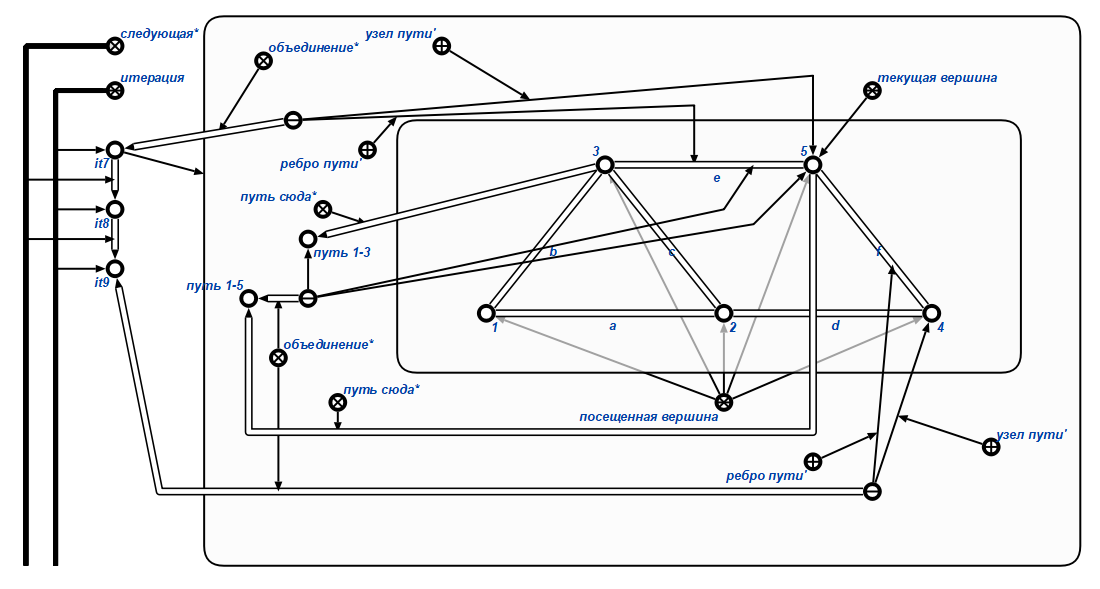
\includegraphics[width=0.45\textwidth]{img/img12.png}
		\caption{Рис.12}
	\end{figure}
% 13
	\item Переходим к ``it8''. Ребро пути - ``f'', вершина пути - ``5''. Эта вершина принадлежит множеству посещенных и путь сюда уже построен, значит итерация игнорируется. Идем дальше.
	\begin{figure}[h]
		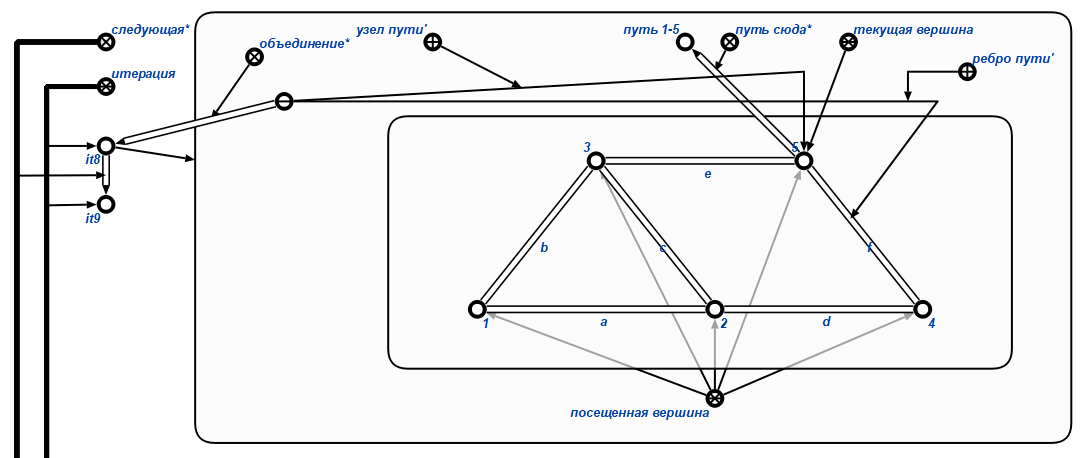
\includegraphics[width=0.45\textwidth]{img/img13.png}
		\caption{Рис.13}
	\end{figure}
% 14
	\item У девятой итерации вершина пути также отмечена посещенной, так что и она тоже игнорируется.
    \newpage
	\begin{figure}[h]
		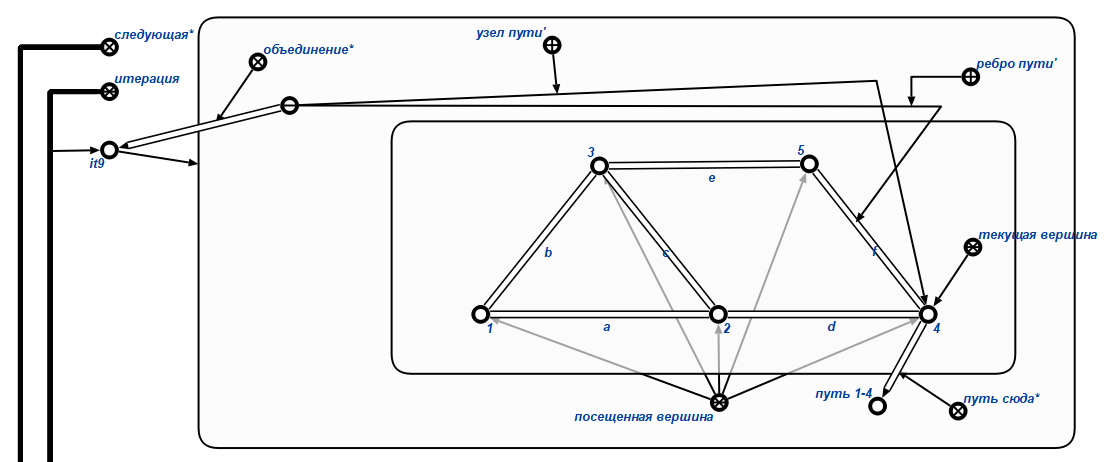
\includegraphics[width=0.45\textwidth]{img/img14.png}
		\caption{Рис.14}
	\end{figure}
% 15
	\item Итак, у нас появилось некоторое количество новых графов ``путь 1-n'', где n - номер крайней вершины графа, то есть каждый такой граф - путь из первой вершины в n-ую. Объединение всех этих путей - есть дерево кратчайших путей исходного графа.
	\begin{figure}[h]
		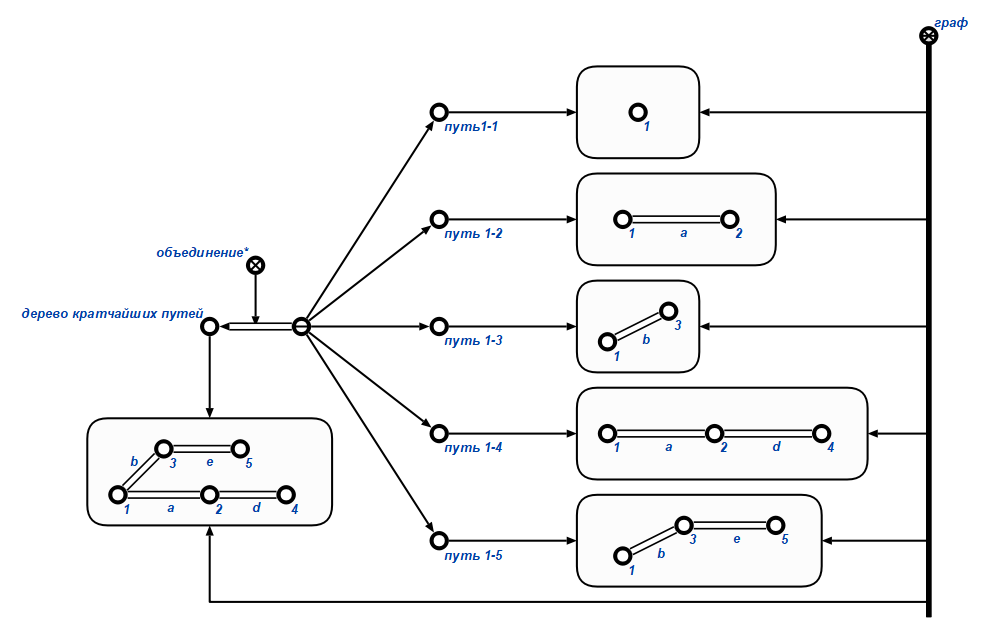
\includegraphics[width=0.45\textwidth]{img/img15.png}
		\caption{Рис.15}
	\end{figure}
\end{enumerate}

\par На рисунках 16-19 представлен вывод работы программы для неориентированного графа, ориентированного графа, взвешенного неориентированного графа, взвешенного ориентированного графа в соответствующем порядке.

% 16
\begin{verbatim}
    ввод:               вывод:
    0 1 1 0             0 1 1 0
    1 0 1 1             0 0 0 1
    1 1 0 0             0 0 0 0
    0 1 0 0             0 0 0 0
\end{verbatim}
\begin{figure}[h]
	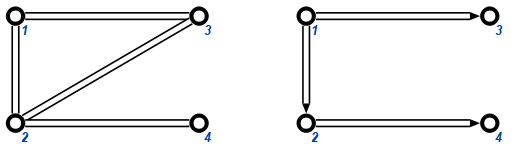
\includegraphics[width=0.45\textwidth]{img/img16.png}
    \caption{Рис.16}
\end{figure}

% 17
\newpage
\begin{verbatim}
  ввод:               вывод:
  0 1 1 0 0           0 1 1 0 0
  0 0 0 1 0           0 0 0 1 0
  0 1 0 0 1           0 0 0 0 1
  0 0 0 0 1           0 0 0 0 0
  0 0 0 0 0           0 0 0 0 0
\end{verbatim}
\begin{figure}[h]
	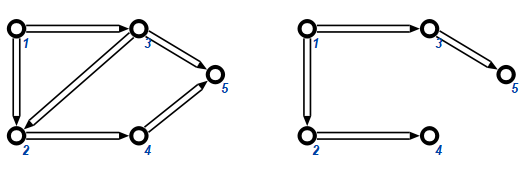
\includegraphics[width=0.45\textwidth]{img/img17.png}
    \caption{Рис.17}
\end{figure}

% 18
\begin{verbatim}
  ввод:               вывод:
  0 3 2 0 0           0 3 2 0 0
  3 0 1 4 0           0 0 0 4 0
  2 1 0 0 5           0 0 0 0 5
  0 4 0 0 2           0 0 0 0 0
  0 0 5 2 0           0 0 0 0 0
\end{verbatim}
\begin{figure}[h]
	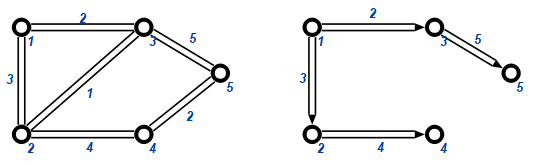
\includegraphics[width=0.45\textwidth]{img/img18.png}
    \caption{Рис.18}
\end{figure}

% 19
\begin{verbatim}
    ввод:               вывод:
    0 6 3 0             0 0 3 0
    0 0 0 1             0 0 0 1
    0 2 0 0             0 2 0 0
    0 0 0 0             0 0 0 0
\end{verbatim}
\begin{figure}[h]
	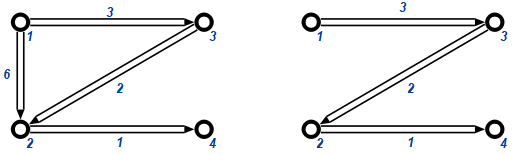
\includegraphics[width=0.45\textwidth]{img/img19.png}
    \caption{Рис.19}
\end{figure}

\newpage
\large{\textbf{Выводы:}}
\par В результате выполнения данной расчётной работы был формализован алгоритм нахождения дерева кротчайших путей невзвешенных неориентированных  и ориентированных графах, были изучены:
\begin{enumerate}
	\item[$\bullet$] Основы теории графов
	\item[$\bullet$] Способы представления графов
	\item[$\bullet$] Базовые алгоритмы для работы с графами
	\item[$\bullet$] Основы SC-кода и SC-алфавита
\end{enumerate}
\large{\textbf{Источники:}}
\begin{enumerate}
	\item[$\bullet$] Оре О. Теория графов. – 2-е изд.. – М.: Наука, 1980. – С. 336.
	\item[$\bullet$] Кормен Т. Х. и др. Часть VI. Алгоритмы для работы с графами // Алгоритмы: построение и анализ = Introduction to Algorithms. – 2-е изд.. – М.: Вильямс, 2006. – С. 1296.
	\item[$\bullet$] Харари, Ф. Теория графов / Ф. Харари / Пер. с англ. и предисл. В.П. Козырева. Под ред. Г.П. Гаврилова. Изд. 2-е. – М.: Едиториал УРСС, 2003. – 269 с.
\end{enumerate}
\end{document}